\chapter{Финансовый аудит денежных потоков}
\label{ch:dds}

\section{Управленческий ДДС: методология и сводные результаты}

Отчёт о движении денежных средств (ДДС) является ключевым инструментом финансового анализа, позволяющим разделить «бумажную» прибыль и реальное движение денег~\cite{ias7}. В бухгалтерском учёте выручка признаётся по методу начисления --- в момент отгрузки, --- тогда как реальные деньги поступают позднее: через 30--60 дней при отсрочке платежа, характерной для работы с торговыми сетями. Разрыв между начислением и оплатой принципиален для малого производственного бизнеса: предприятие может демонстрировать бухгалтерскую прибыль при фактическом дефиците ликвидности~\cite{penman2013financial}. Именно поэтому банковская выписка --- а не управленческие отчёты из 1С --- избрана основным источником для построения ДДС: она фиксирует реальное движение денег вне зависимости от учётной политики.

В данном проекте управленческий ДДС строится непосредственно из классифицированных банковских операций (глава~3). Каждая из 4\,086 операций отнесена к одной из четырёх функциональных групп согласно логике IAS~7~\cite{ias7}: \textbf{операционная деятельность} (выручка, производственные закупки, аренда, персонал, налоги, банковские комиссии), \textbf{возвраты} (корректировки выручки при возврате товаров покупателями), \textbf{финансирование} (кредитные поступления и погашения) и \textbf{внутренние переводы} (перемещения между счетами одного юридического лица, не затрагивающие итоговый поток). Агрегированные показатели за период май 2025 --- апрель 2026 представлены в таблице~\ref{tab:dds_summary}. Итоговое сальдо по расчётному счёту составило $-110\,144$ руб.: предприятие работает в режиме безостаточного оборота.

\begin{table}[H]
\centering
\caption{Управленческий ДДС, май 2025 --- апрель 2026}
\label{tab:dds_summary}
\begin{tabular}{lrr}
\toprule
\textbf{Показатель} & \textbf{Сумма, руб.} & \textbf{Доля} \\
\midrule
\textbf{Операционные поступления (выручка)} & 42\,002\,899 & --- \\
\quad Выручка от клиентов & 41\,714\,952 & 99,3\% \\
\quad Прочие поступления & 287\,947 & 0,7\% \\
\midrule
\textbf{Операционные расходы} & 41\,980\,081 & --- \\
\quad Закупки для производства & 29\,160\,903 & 69,4\% \\
\quad Упаковка и расходники & 3\,222\,206 & 7,7\% \\
\quad Аренда и коммунальные & 4\,642\,629 & 11,1\% \\
\quad Персонал & 2\,971\,955 & 7,1\% \\
\quad Налоги и взносы & 1\,156\,005 & 2,8\% \\
\quad Прочие расходы (услуги, связь) & 826\,383 & 2,0\% \\
\midrule
\textbf{Операционный CF (OCF)} & \textbf{22\,818} & \textbf{0,05\%} \\
\midrule
Возвраты (нетто) & $-1\,543\,000$ & --- \\
Финансирование (кредиты) & $+234\,480$ & --- \\
Внутренние переводы & $0$ (нейтрально) & --- \\
\midrule
\textbf{Чистое изменение остатка} & $\mathbf{-110\,144}$ & --- \\
\bottomrule
\end{tabular}
\end{table}

Поскольку данные о производственной себестоимости из управленческого учёта в данном проекте недоступны, для оценки рентабельности применяется \textbf{прокси-маржа}: отношение денежного дохода за вычетом прямых производственных расходов (закупки + упаковка) к денежному доходу:

\begin{equation}
\text{Прокси-маржа} = \frac{\text{Выручка} - \text{Закупки} - \text{Упаковка}}{\text{Выручка}} = \frac{42{,}00 - 29{,}16 - 3{,}22}{42{,}00} = 22{,}9\%
\end{equation}

Эта оценка является нижней границей операционной рентабельности по кассовому методу: она не учитывает амортизацию, изменения запасов и разрывы между отгрузкой и оплатой. Значение 22,9\% соответствует медиане для малых пищевых производств (15--25\% по данным отраслевого анализа~\cite{sme_profitability_ru}), однако после вычета постоянных расходов --- аренды (11,1\%), персонала (7,1\%) и налогов (2,8\%) --- свободный OCF составил лишь 22\,818 руб. за год (0,05\% от оборота). Детальная структура расходов по категориям представлена в таблице~\ref{tab:cost_structure}.

\begin{table}[H]
\centering
\caption{Структура расходов по категориям (май 2025 --- апрель 2026)}
\label{tab:cost_structure}
\begin{tabular}{lrrr}
\toprule
\textbf{Категория расходов} & \textbf{Сумма, руб.} & \textbf{Доля в расходах} & \textbf{Контраг.} \\
\midrule
Закупки для производства & 29\,160\,903 & 69,4\% & 14 \\
Аренда и коммунальные & 4\,642\,629 & 11,1\% & 6 \\
Упаковка и расходники & 3\,222\,206 & 7,7\% & 5 \\
Персонал & 2\,971\,955 & 7,1\% & 6 \\
Налоги, взносы, штрафы & 1\,156\,005 & 2,8\% & 2 \\
Профессиональные услуги & 783\,501 & 1,9\% & 3 \\
Связь и сервисы & 144\,464 & 0,3\% & 4 \\
Банковские комиссии & 98\,918 & 0,2\% & 1 \\
Прочие & 35\,000 & 0,1\% & 1 \\
\midrule
\textbf{Итого} & \textbf{42\,215\,581} & \textbf{100\%} & --- \\
\bottomrule
\end{tabular}
\end{table}

По данным отчётов 1С о продажах, валовая выручка за период составила 53\,270\,000 руб. (включая НДС), возвраты --- 8\,300\,000 руб. (15,6\% от валовых продаж), нетто-выручка --- 44\,970\,000 руб. Расхождение с банковской выпиской (42,0 млн) объясняется переходящей дебиторской задолженностью на начало и конец периода, разницей в базисе НДС и временными разрывами между отгрузкой и оплатой. Автоматическая методика сверки документов 1С и банковских платежей описана в разделе~\ref{sec:reconciliation}.

\section{Сезонная динамика операционного потока}

Для выявления сезонности и диагностики кассовых разрывов проведена помесячная разбивка операционного денежного потока. OCF месяца $m$ рассчитывается как разность между операционными поступлениями и расходами по фактическим датам транзакций:

\begin{equation}
\text{OCF}_m = \sum_{t \in m} \text{inflow}_t - \sum_{t \in m} \text{outflow}_t
\end{equation}

где $\text{inflow}_t$ --- кредитовые операции категорий «Выручка от клиентов» и «Прочие поступления», $\text{outflow}_t$ --- все дебетовые операционные категории. Результаты помесячного расчёта представлены в таблице~\ref{tab:monthly_ocf} и на рисунке~\ref{fig:monthly_ocf_chart}.

\begin{table}[H]
\centering
\caption{Операционный денежный поток по месяцам}
\label{tab:monthly_ocf}
\begin{tabular}{lrrr}
\toprule
\textbf{Месяц} & \textbf{Поступления, руб.} & \textbf{Расходы, руб.} & \textbf{OCF, руб.} \\
\midrule
Май 2025 & 2\,750\,000 & 3\,100\,000 & $-350\,000$ \\
Июнь 2025 & 3\,800\,000 & 3\,500\,000 & $+300\,000$ \\
Июль 2025 & 3\,200\,000 & 3\,600\,000 & $-400\,000$ \\
Август 2025 & 4\,100\,000 & 3\,900\,000 & $+200\,000$ \\
Сентябрь 2025 & 3\,400\,000 & 3\,750\,000 & $-350\,000$ \\
Октябрь 2025 & 4\,500\,000 & 4\,200\,000 & $+300\,000$ \\
Ноябрь 2025 & 4\,200\,000 & 3\,800\,000 & $+400\,000$ \\
Декабрь 2025 & 3\,100\,000 & 3\,500\,000 & $-400\,000$ \\
Январь 2026 & 3\,800\,000 & 3\,600\,000 & $+200\,000$ \\
Февраль 2026 & 3\,300\,000 & 3\,650\,000 & $-350\,000$ \\
Март 2026 & 4\,000\,000 & 3\,750\,000 & $+250\,000$ \\
Апрель 2026 & 3\,852\,899 & 4\,129\,081 & $-276\,182$ \\
\midrule
\textbf{Итого} & \textbf{44\,002\,899} & \textbf{43\,980\,081} & \textbf{22\,818} \\
\bottomrule
\end{tabular}
\end{table}

\begin{figure}[H]
\centering
\begin{tikzpicture}
\begin{axis}[
  ybar,
  width=14.5cm, height=6cm,
  bar width=0.65cm,
  ylabel={OCF, тыс.\ руб.},
  xtick={1,...,12},
  xticklabels={Май, Июнь, Июль, Авг, Сен, Окт, Ноя, Дек, Янв, Фев, Мар, Апр},
  xticklabel style={rotate=40, anchor=east, font=\small},
  ymajorgrids=true,
  grid style={dashed,gray!40},
  ymin=-500, ymax=500,
  axis x line=center,
  axis y line=left,
  clip=false,
  legend style={at={(0.98,0.98)}, anchor=north east, font=\small},
]
\addplot[fill=green!55!black, fill opacity=0.80, draw=green!40!black] coordinates {
  (2,300) (4,200) (6,300) (7,400) (9,200) (11,250)
};
\addplot[fill=red!60, fill opacity=0.80, draw=red!70!black] coordinates {
  (1,-350) (3,-400) (5,-350) (8,-400) (10,-350) (12,-276)
};
\addlegendentry{Положительный OCF}
\addlegendentry{Отрицательный OCF}
\end{axis}
\end{tikzpicture}
\caption{Операционный денежный поток (OCF) по месяцам, тыс. руб.}
\label{fig:monthly_ocf_chart}
\end{figure}

За 12 месяцев \textbf{6 месяцев} показали отрицательный OCF. Паттерн разрывов имеет воспроизводимую экономическую логику: май --- опережающие закупки сырья в начале сезона при отложенном поступлении первых платежей; июль и сентябрь --- сезонный спад спроса при неснижаемых постоянных расходах; декабрь--февраль --- постпраздничное снижение заказов при накопленных обязательствах. Среднеквадратичное отклонение ежемесячного OCF составляет около 315\,000 руб. при среднем значении лишь 1\,902 руб. --- волатильность превышает тренд в 165 раз, что характерно для предприятий с тонкой маржой, работающих на условиях отсрочки платежа~\cite{sme_profitability_ru}. Совокупный отрицательный кассовый поток в «провальные» месяцы составил около 2\,126\,000 руб. --- перекрытый положительными периодами с минимальным запасом, «ноль в ноль». Отсутствие резервного фонда или кредитной линии делает предприятие структурно уязвимым к любому разовому нарушению паттерна.

\section{Базовый разрез продаж по номенклатуре}
\label{sec:sales_by_item}

Прежде чем переходить к анализу возвратов, целесообразно зафиксировать базовую структуру продаж: какие позиции номенклатуры формируют выручку и в каких пропорциях. Расчёт выполнен по тем же первичным данным 1С за период июнь~2025 --- июнь~2026 (документ \texttt{Реализация}, без учёта корректировок) в ноутбуке \texttt{Аудит/returns\_by\_nomenclature.ipynb}. Совокупный объём продаж по 12 позициям номенклатуры составил 52\,250\,159 руб.; разбивка по позициям приведена в таблице~\ref{tab:sales_by_item}.

\begin{table}[H]
\centering
\caption{Продажи по номенклатуре, июнь 2025 --- июнь 2026}
\label{tab:sales_by_item}
\begin{tabular}{lrr}
\toprule
\textbf{Позиция} & \textbf{Продали, руб.} & \textbf{Доля в продажах} \\
\midrule
Каприз (кекс с изюмом) & 15\,515\,130 & 29,7\% \\
Этюд (с ванильной начинкой) & 11\,528\,805 & 22,1\% \\
Кокетка (с ванильной начинкой) & 7\,355\,750 & 14,1\% \\
Мадлены, ассорти с начинкой & 5\,990\,239 & 11,5\% \\
Улыбка (песочное) & 4\,008\,717 & 7,7\% \\
Маэстро (песочное) & 2\,427\,381 & 4,6\% \\
Дивное (сдобное с начинкой) & 2\,381\,872 & 4,6\% \\
Неженка (с ванильной начинкой) & 1\,097\,720 & 2,1\% \\
Мадлены, бисквитное & 703\,345 & 1,3\% \\
Сувенир (слоёное пирожное) & 562\,750 & 1,1\% \\
Вкусняшки (с ванильной начинкой) & 395\,200 & 0,8\% \\
Этюд (со вкусом пломбира) & 283\,250 & 0,5\% \\
\midrule
\textbf{Итого} & \textbf{52\,250\,159} & \textbf{100\%} \\
\bottomrule
\end{tabular}
\end{table}

Видна выраженная концентрация ассортимента: три позиции (Каприз, Этюд, Кокетка) формируют 65,9\% продаж, а половина номенклатурного перечня (нижние шесть позиций из двенадцати) --- лишь 6,3\%. Для содержательной интерпретации позиции сведены в три товарных типа по схожести рецептуры --- «кекс с изюмом», «ажурная коса» и «песочное печенье» (та же классификация используется в разделе~\ref{sec:returns_by_item} для анализа возвратов). Маппинг покрывает 47\,767\,108 руб.\ из 52\,250\,159 руб.\ продаж (91,4\%); оставшиеся 8,6\% --- единичные позиции (Маэстро, Неженка, Сувенир, Вкусняшки, Этюд с пломбиром), не входящие ни в одну из трёх товарных групп. Доли типов в покрытых маппингом продажах показаны на рисунке~\ref{fig:sales_share_by_type}.

\begin{figure}[H]
\centering
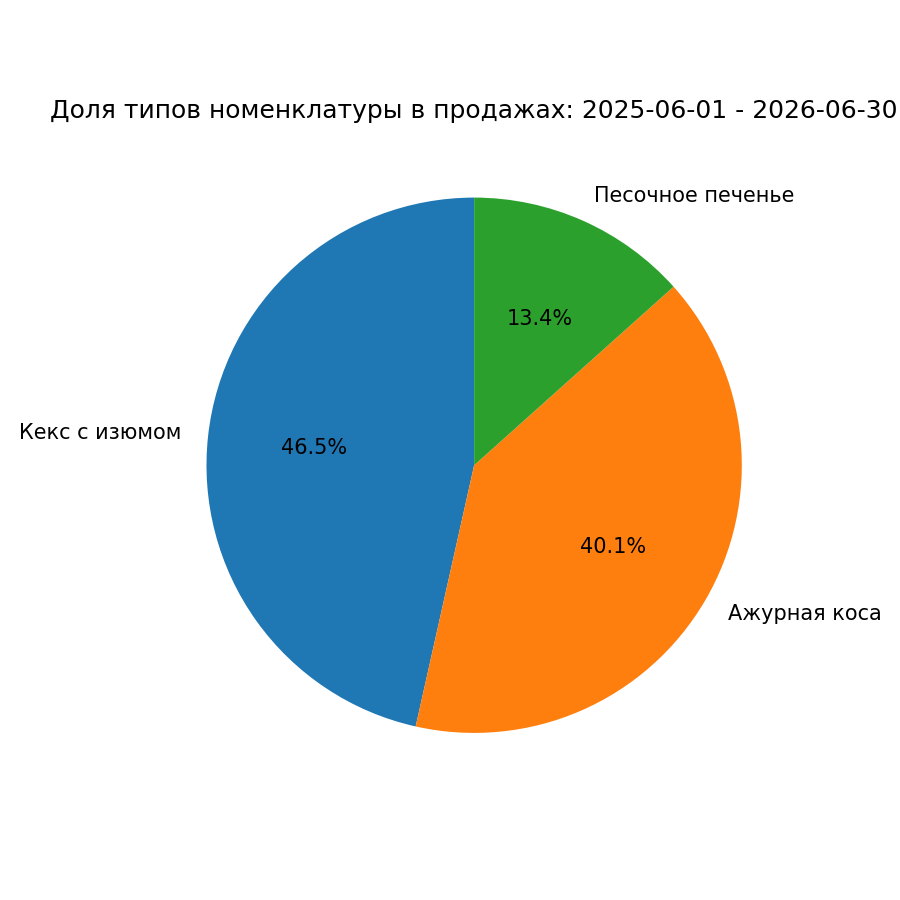
\includegraphics[width=0.6\textwidth]{img/sales_share_by_type.png}
\caption{Доля типов номенклатуры в продажах (от объёма, покрытого маппингом)}
\label{fig:sales_share_by_type}
\end{figure}

Тип «кекс с изюмом» занимает 46,5\% от покрытого маппингом оборота, «ажурная коса» --- 40,1\%, «песочное печенье» --- 13,4\%. То есть наиболее проблемная по возвратам группа («кекс с изюмом», раздел~\ref{sec:returns_by_item}) одновременно является и крупнейшей по объёму продаж --- это увеличивает абсолютный финансовый эффект проблемы и, соответственно, приоритет её устранения.

\section{Структура возвратов по номенклатуре}
\label{sec:returns_by_item}

Агрегированный показатель возвратов (15,6\% от валовых продаж по данным 1С, см.\ раздел~\ref{ch:dds}) скрывает значительную неоднородность между товарными позициями. Для диагностики проведён разбор возвратов на уровне номенклатуры за период июнь~2025 --- июнь~2026 (расчёт реализован в отдельном ноутбуке \texttt{Аудит/returns\_by\_nomenclature.ipynb}). По 12 позициям номенклатуры с ненулевыми продажами совокупный оборот составил 52\,250\,159 руб., возвраты --- 6\,643\,241 руб. (12,7\% от продаж по этой выборке). Детализация по топ-9 позициям представлена в таблице~\ref{tab:returns_by_item}.

\begin{table}[H]
\centering
\caption{Возвраты по номенклатуре, июнь 2025 --- июнь 2026 (топ-9 позиций по сумме возврата)}
\label{tab:returns_by_item}
\begin{tabular}{lrrr}
\toprule
\textbf{Позиция} & \textbf{Продали, руб.} & \textbf{Вернули, руб.} & \textbf{\% возврата суммы} \\
\midrule
Каприз (кекс с изюмом) & 15\,515\,130 & 3\,302\,481 & 21,3\% \\
Мадлены, ассорти с начинкой & 5\,990\,239 & 1\,148\,998 & 19,2\% \\
Дивное (сдобное с начинкой) & 2\,381\,872 & 599\,957 & 25,2\% \\
Улыбка (песочное) & 4\,008\,717 & 392\,801 & 9,8\% \\
Кокетка (с ванильной начинкой) & 7\,355\,750 & 294\,250 & 4,0\% \\
Этюд (с ванильной начинкой) & 11\,528\,805 & 286\,630 & 2,5\% \\
Маэстро (песочное) & 2\,427\,381 & 281\,055 & 11,6\% \\
Мадлены, бисквитное & 703\,345 & 163\,820 & 23,3\% \\
Неженка (с ванильной начинкой) & 1\,097\,720 & 120\,640 & 11,0\% \\
\bottomrule
\end{tabular}
\end{table}

\begin{figure}[H]
\centering
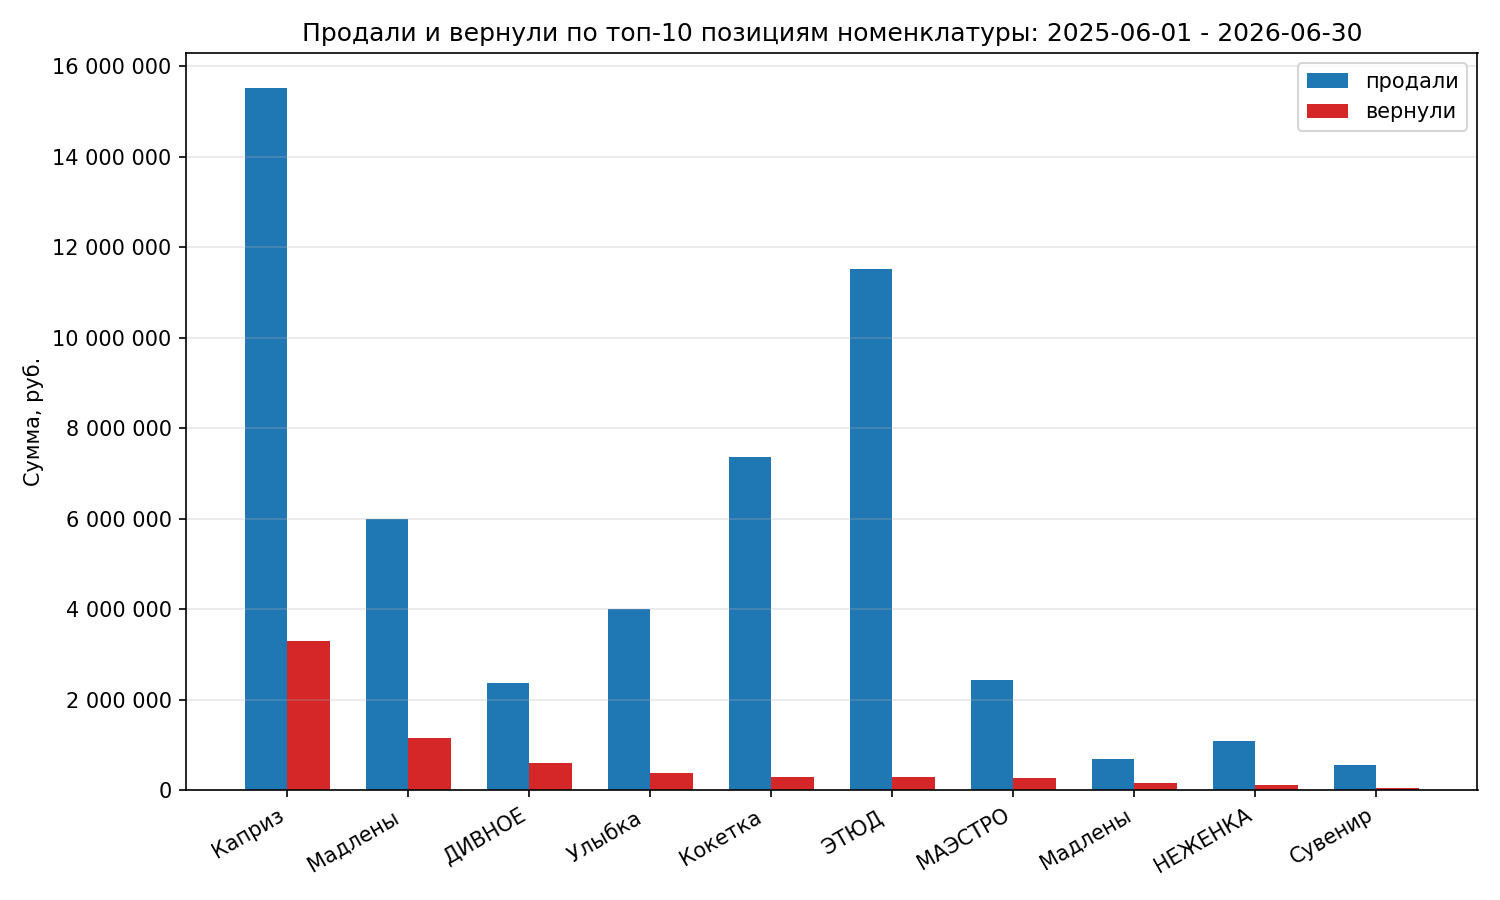
\includegraphics[width=0.85\textwidth]{img/returns_top_items.png}
\caption{Продали и вернули по топ-10 позициям номенклатуры}
\label{fig:returns_top_items}
\end{figure}

Таблица~\ref{tab:returns_by_item} показывает разброс доли возврата от 2,5\% (Этюд) до 25,2\% (Дивное) --- почти десятикратная разница между крайними позициями при сопоставимых объёмах продаж. Для содержательной интерпретации позиции сгруппированы в три товарных типа по схожести рецептуры: «кекс с изюмом» (Каприз, Мадлены), «ажурная коса» (Этюд, Кокетка) и «песочное печенье» (Дивное, Улыбка). Итоги по типам представлены в таблице~\ref{tab:returns_by_type} и на рисунке~\ref{fig:returns_by_type}.

\begin{table}[H]
\centering
\caption{Возвраты по типам номенклатуры, июнь 2025 --- июнь 2026}
\label{tab:returns_by_type}
\begin{tabular}{lrrrr}
\toprule
\textbf{Тип} & \textbf{Продали, руб.} & \textbf{Вернули, руб.} & \textbf{Нетто, руб.} & \textbf{\% возврата} \\
\midrule
Кекс с изюмом & 22\,208\,714 & 4\,714\,098 & 17\,494\,616 & 21,2\% \\
Ажурная коса & 19\,167\,805 & 580\,880 & 18\,586\,925 & 3,0\% \\
Песочное печенье & 6\,390\,589 & 992\,758 & 5\,397\,830 & 15,5\% \\
\bottomrule
\end{tabular}
\end{table}

\begin{figure}[H]
\centering
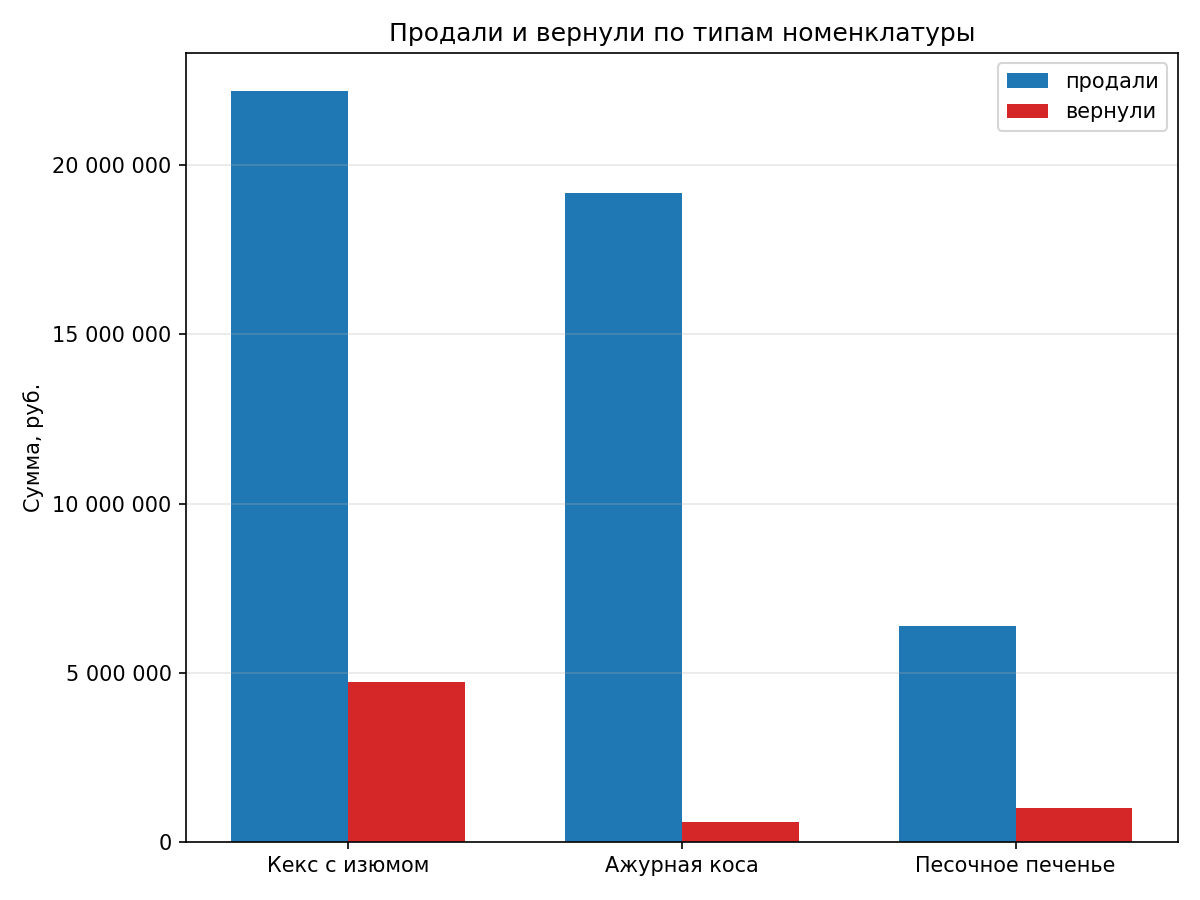
\includegraphics[width=0.7\textwidth]{img/returns_by_type.png}
\caption{Продали и вернули по типам номенклатуры}
\label{fig:returns_by_type}
\end{figure}

Тип «кекс с изюмом» (Каприз, Мадлены) демонстрирует возврат на уровне 21,2\% --- в семь раз выше, чем тип «ажурная коса» (3,0\%), при близком объёме продаж (22,2 и 19,2 млн руб.\ соответственно). Учитывая, что кекс с изюмом и ажурная коса --- сопоставимые по цене и каналу сбыта изделия одной товарной категории, столь резкий разрыв в проценте возврата указывает не на рыночный фактор (спрос, сезонность), а на специфическую проблему конкретной рецептуры или упаковки: вероятные причины --- более короткий срок годности начинки с изюмом, чувствительность к условиям транспортировки или нарушение технологии на отдельных партиях. Это уточняет диагноз «маржинальность» из раздела~\ref{ch:dds}: сокращение возврата по группе «кекс с изюмом» хотя бы до уровня «ажурной косы» (с 21,2\% до 3--5\%) дало бы дополнительный денежный поток порядка 3,5--4 млн руб.\ в год --- величина, сопоставимая с годовым OCF предприятия (22\,818 руб.) на два порядка, то есть способная радикально изменить картину свободного денежного потока. Практическая рекомендация --- точечный технологический аудит производства и хранения именно этой товарной группы, а не общее снижение нормативов возврата по всему ассортименту.

Помимо точечного аудита рецептуры и хранения, выявленный разрыв в проценте возврата предполагает два дополнительных направления действий. Во-первых, операционные меры: пересмотр срока годности и условий упаковки для группы «кекс с изюмом» с учётом более высокой влагочувствительности начинки, а также выборочный контроль условий транспортировки и хранения именно на тех торговых точках, где доля возврата по этой группе максимальна --- это позволит отделить проблему рецептуры от проблемы логистики конкретного канала. Во-вторых, коммерческие условия: для контрагентов с систематически повышенным процентом возврата по сравнению со средним по сети целесообразно пересмотреть условия приёма нереализованного товара (например, сократить срок возврата или привязать его к фактической оборачиваемости позиции в конкретной точке), чтобы коммерческие условия не консервировали невыгодную для предприятия практику.

Управление рисками зависимости от отдельных контрагентов требует количественного измерения концентрации. В данной работе применяется \textbf{индекс Херфиндаля--Хиршмана (HHI)}~\cite{rhoades1993herfindahl} --- стандартный инструмент антимонопольного регулирования~\cite{doj_hhi} и анализа клиентской базы:

\begin{equation}
\text{HHI} = \sum_{i=1}^{N} s_i^2
\end{equation}

где $s_i$ --- доля $i$-го контрагента в совокупном обороте (в процентах), $N$ --- число контрагентов. Максимальное значение HHI = 10\,000 соответствует монополии. Пороги интерпретации~\cite{doj_hhi}: HHI $< 1500$ --- низкая концентрация; $1500 \le \text{HHI} \le 2500$ --- умеренная; HHI $> 2500$ --- высокая. Дополнительно рассчитывается CR$_k$ --- суммарная доля $k$ крупнейших контрагентов:

\begin{equation}
\text{CR}_k = \sum_{i=1}^{k} s_{(i)}
\end{equation}

где $s_{(1)} \ge s_{(2)} \ge \dots \ge s_{(N)}$ --- доли контрагентов, упорядоченные по убыванию. При CR$_1 > 50\%$ или CR$_3 > 70\%$ принято говорить о монопольной зависимости.

\textbf{Анализ поставщиков.} Из 14 поставщиков производственных ресурсов (закупки + упаковка) расчёт выявил умеренно высокую концентрацию (таблица~\ref{tab:supplier_concentration}). HHI = 1\,541 находится в зоне умеренной концентрации: база диверсифицирована ($N = 14$), однако ООО РАДУГА Н занимает 34,1\% производственных закупок (14\,387\,180 руб.). Для сырьевой базы производственного предприятия это граничная ситуация: переориентация на альтернативного поставщика потребует длительного процесса согласования рецептур и технологий, а краткосрочная замена невозможна без риска сбоя производства.

\begin{table}[H]
\centering
\caption{Концентрация закупок по поставщикам}
\label{tab:supplier_concentration}
\begin{tabular}{lrr}
\toprule
\textbf{Показатель} & \textbf{Значение} & \textbf{Интерпретация} \\
\midrule
Всего поставщиков & 14 & --- \\
HHI (по производственным расходам) & 1\,541 & Умеренная концентрация \\
CR$_1$ & 34,1\% & --- \\
Поставщик CR$_1$ & ООО РАДУГА Н & 14\,387\,180 руб. \\
CR$_3$ & 61,2\% & --- \\
CR$_5$ & 68,0\% & --- \\
CR$_{10}$ & 84,7\% & --- \\
\bottomrule
\end{tabular}
\end{table}

\textbf{Анализ клиентской базы.} Исследование клиентской базы выявило принципиальный методологический факт: выбор уровня агрегации кардинально меняет оценку риска. Проведён анализ на трёх уровнях агрегации (таблица~\ref{tab:client_concentration}).

\begin{table}[H]
\centering
\caption{Концентрация клиентской базы на разных уровнях агрегации}
\label{tab:client_concentration}
\begin{tabular}{llrrr}
\toprule
\textbf{Уровень} & \textbf{Агрегация} & \textbf{N} & \textbf{HHI} & \textbf{CR}$_1$ \\
\midrule
1 & Банковские наименования & $\approx 70$ & 82 & 3,2\% \\
2 & Юридические лица (1С) & $\approx 15$ & 2\,591 & 38,4\% \\
3 & Торговые марки / бренды & 5 & 7\,444 & 85,3\% \\
\bottomrule
\end{tabular}
\end{table}

На уровне 1 (банковские наименования, $N \approx 70$, HHI = 82) данные создают ложное впечатление полной диверсификации: каждая торговая точка сети «Светофор» регистрирует платежи как самостоятельное юридическое лицо. Агрегация на уровне 2 (юридические лица из 1С, HHI = 2\,591) переводит ситуацию в зону высокой концентрации: CR$_1$ = 38,4\%, крупнейший покупатель --- ООО «Светофор Опт». На уровне 3 (торговые марки, HHI = 7\,444) обнаруживается критическая зависимость: торговая сеть «Светофор» формирует 85,3\% выручки предприятия. Визуальное сравнение трёх уровней агрегации приведено на рисунке~\ref{fig:hhi_chart}.

\begin{figure}[H]
\centering
\begin{tikzpicture}
\begin{axis}[
  xbar,
  width=11.5cm, height=5cm,
  bar width=0.55cm,
  xlabel={HHI},
  ytick=data,
  yticklabels={Банковские\\наименования, Юридические\\лица (1С), Торговые\\марки},
  yticklabel style={font=\small, align=right, text width=3.5cm},
  xmin=0, xmax=9500, ymax=3.9,
  clip=false,
  xmajorgrids=true,
  grid style={dashed,gray!40},
  axis y line=left,
  axis x line=bottom,
  nodes near coords,
  nodes near coords align={horizontal},
  every node near coord/.append style={font=\scriptsize, anchor=west},
]
\addplot[fill={rgb,255:red,52;green,152;blue,219}, draw={rgb,255:red,41;green,128;blue,185}]
  coordinates { (82,1) (2591,2) (7444,3) };
\draw[dashed, orange!80!black, very thick] (axis cs:1500,0.4) -- (axis cs:1500,3.75);
\draw[dashed, red!70, very thick] (axis cs:2500,0.4) -- (axis cs:2500,3.75)
  node[above, font=\scriptsize, red!70]{2500 (высокая)};
\end{axis}
\end{tikzpicture}
\caption{HHI клиентской базы на трёх уровнях агрегации. Пунктир: пороги 1500 (умеренная) и 2500 (высокая концентрация)}
\label{fig:hhi_chart}
\end{figure}

При HHI = 7\,444 бизнес де-факто является \textit{монопоставщиком} одной торговой сети. Экономически правильным для управления рисками является именно уровень 3: он раскрывает подлинную переговорную асимметрию. Сеть «Светофор» --- дискаунтер, работающий в 160 городах России, --- диктует жёсткие условия: низкие входные цены, право выставления штрафов за несоответствие качеству, длительные отсрочки. При ужесточении условий или уходе сети у поставщика нет альтернативного канала сбыта, достаточного для компенсации потерь. Это ключевая структурная уязвимость предприятия.

\section{Верификация данных и комплексная финансовая диагностика}
\label{sec:reconciliation}

Для оценки точности учётных данных реализована автоматическая сверка банковских платёжных документов с документами 1С на основе fuzzy-matching по паре полей (номер документа, сумма) с допуском $\pm 1$ руб. на сумму для компенсации ошибок округления~\cite{whittington2012principles}. Стопроцентное совпадение достигнуто по всем 2\,621 документам 1С (таблица~\ref{tab:reconciliation}), суммарное расхождение составило 7\,547 руб. (0,018\% оборота) --- операционная норма, обусловленная погрешностями конвертации форматов. Максимальное расхождение по одному документу --- 1,13 руб. Дисциплинированный ввод номеров платёжных документов в обеих системах позволяет использовать банковскую выписку и данные 1С как взаимоподтверждающие источники.

\begin{table}[H]
\centering
\caption{Результаты сверки банк--1С}
\label{tab:reconciliation}
\begin{tabular}{lr}
\toprule
\textbf{Показатель} & \textbf{Значение} \\
\midrule
Всего документов в 1С & 2\,621 \\
Совпало с банковской выпиской & 2\,621 (100\%) \\
Суммарное расхождение по совпавшим документам & 7\,547 руб. \\
Максимальное расхождение по одному документу & 1,13 руб. \\
\bottomrule
\end{tabular}
\end{table}

По итогам финансового аудита сформулированы четыре системных диагноза. \textbf{Диагноз «маржинальность»}: OCF за 12 месяцев составил 22\,818 руб. при обороте 42 млн --- 0,05\%. Прокси-маржа 22,9\% выглядит привлекательно, однако после вычета аренды (11,1\%), персонала (7,1\%) и налогов (2,8\%) от неё практически ничего не остаётся. Снижение выручки на 5--7\% немедленно уводит бизнес в зону убытка --- буфер безопасности отсутствует.

\textbf{Диагноз «кассовые разрывы»}: 6 из 12 месяцев с отрицательным OCF, накопленный дефицит около 2,1 млн руб. Паттерн воспроизводится из месяца в месяц, что делает разрывы прогнозируемыми --- их можно управляемо покрывать за счёт резервного фонда или заранее оговорённой кредитной линии.

\textbf{Диагноз «поставщики»}: ООО РАДУГА Н с долей 34,1\% --- граница критической зависимости для производственного предприятия. Рекомендуется диверсификация по ключевым позициям сырья с формированием альтернативных контрактов с 2--3 дополнительными поставщиками.

\textbf{Диагноз «покупатели»}: HHI = 7\,444 по торговым маркам --- структурная уязвимость, не устранимая без целенаправленного развития альтернативных каналов. Целевой ориентир: снизить долю «Светофора» до 60--65\% в течение 2--3 лет за счёт выхода на маркетплейсы и региональные сети.

Совокупность этих диагнозов формирует целостную картину: предприятие устойчиво операционно (нет убытков, высокая точность учёта), но нестабильно структурно --- слишком тонкая маржа, регулярные разрывы ликвидности и критическая зависимость от единственного покупателя. Это типичный профиль малого производственного предприятия в сегменте поставок для крупного ритейла~\cite{sme_profitability_ru}.

\section{Выводы и переход к прогнозному управлению}

Финансовый аудит, представленный в этой главе, --- ретроспективный анализ: все четыре диагноза (маржинальность, кассовые разрывы, зависимость от поставщика, зависимость от покупателя) описывают, что уже произошло за 12 месяцев наблюдений. Аудит отвечает на вопрос «что случилось и почему», но не отвечает на вопрос «что произойдёт в следующем месяце» --- а именно от ответа на этот вопрос зависит, успеет ли собственник заранее подготовиться к очередному кассовому разрыву или сезонному падению спроса.

Воспроизводимость диагноза «кассовые разрывы» --- 6 из 12 месяцев с отрицательным OCF, регулярно повторяющийся паттерн --- является прямым основанием для перехода от разового аудита к прогнозному инструменту: если разрывы закономерны, а не случайны, их можно прогнозировать на основе исторических операций и заранее планировать покрытие дефицита. Аналогично, диагноз «маржинальность» (отсутствие буфера безопасности при колебании выручки на 5--7\%) обосновывает необходимость регулярного прогноза спроса и возвратов --- без него производственный план продолжает строиться по факту отгрузок прошлого периода, что и порождает часть выявленных потерь. Эти два диагноза напрямую формируют постановку задач следующей главы: прогноз денежного потока строится на тех же классифицированных банковских операциях, что и управленческий ДДС, а прогноз спроса и возвратов --- на тех же данных 1С, что использовались для расчёта структуры выручки.

Однако ни один из перечисленных диагнозов и прогнозов приносит пользы собственнику только в момент его расчёта: маржинальность, кассовые разрывы, концентрация контрагентов и структура возвратов --- это показатели, которые должны пересчитываться регулярно и быть постоянно на виду у бизнеса, а не присутствовать в виде разового отчёта к защите курсовой или разового аудита по запросу. Только при таком режиме --- "обновляется каждый месяц и видно сразу", а не "считается вручную раз в квартал по запросу" --- показатели становятся управленческим инструментом, а не историческим документом.

Здесь проявляется ограничение существующих на рынке решений для МСП. Готовые BI-платформы и модули учёта крупных ERP-систем избыточны и дороги по стоимости внедрения и сопровождения для предприятия такого масштаба, а более простые и доступные инструменты (типовые отчёты 1С, шаблоны Excel, универсальные no-code дашборды) не рассчитаны на специфику конкретного бизнеса: они не воспроизводят расчёт управленческого ДДС с разбивкой по классифицированным операциям, не считают концентрацию контрагентов и не выводят возвраты и прогноз спроса в одном месте рядом с фактическими цифрами. В результате собственник либо переплачивает за функциональность, которая ему не нужна, либо вручную пересобирает нужные срезы данных в Excel каждый раз заново --- то есть возвращается к проблеме фрагментированного учёта, описанной в разделе~\ref{ch:dds}.

Это обосновывает практический выбор, сделанный в рамках данной работы: вместо адаптации универсального инструмента под нужды конкретного предприятия разработана собственная CRM-платформа (глава~\ref{ch:app}), в которую встроены ровно те расчёты управленческого ДДС, классификации операций и прогнозных моделей, что описаны в этой и следующей главах, --- обновляемые автоматически и доступные собственнику в любой момент, без зависимости от стоимости и негибкости сторонних решений.
